\documentclass{standalone}
\usepackage{tikz}
\usepackage{nono}
\begin{document}
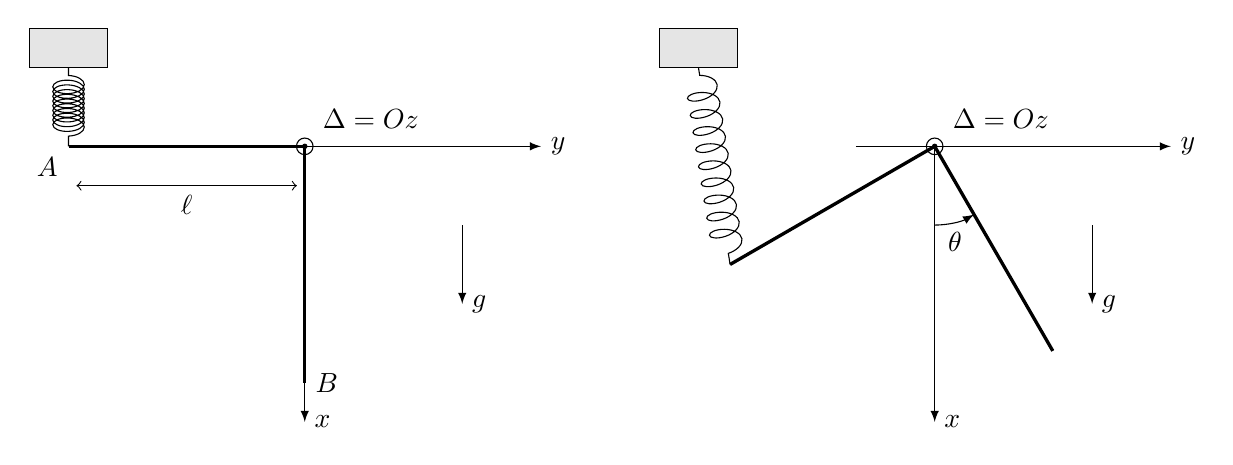
\begin{tikzpicture}
  \draw[-latex] (0, 0) coordinate (O) -- (0,-3.5) node[right]{$x$}; 
  \draw[-latex] (-1, 0) -- (3,0) node[right]{$y$}; 
  \fill (O) circle (1pt);
  \draw (O) circle (3pt) node[above right=3pt]{$\Delta = Oz$};
  % Solide
  \draw[very thick] (O) -- ++(-3,0) node[below left]{$A$} ;
  \draw[very thick] (O) -- ++(0,-3) node[right]{$B$} ;

  % support ressort
  \draw[fill=gray!20] (-3.5, 1)rectangle (-2.5, 1.5);
  \draw[decorate, decoration={coil, amplitude=2mm,segment length=0.6mm,aspect=0.5, post length=1mm, pre length=1mm}] (-3, 1) -- (-3, 0);

  \draw[<->] (-0.1, -0.5) -- (-2.9, -0.5) node[midway, below]{$\ell$}; 

  \draw[-latex] (2, -1) -- ++(0, -1) node[right] {$\vv{g}$}; 

  \begin{scope}[xshift=8cm]
    \draw[-latex] (0, 0) coordinate (O) -- (0,-3.5) node[right]{$x$}; 
    \draw[-latex] (-1, 0) -- (3,0) node[right]{$y$}; 
    \fill (O) circle (1pt);
    \draw (O) circle (3pt) node[above right=3pt]{$\Delta = Oz$};
    % Solide
    \draw[very thick] (O) -- ++(210:3) coordinate(B);
    \draw[very thick] (O) -- ++(-60:3);
    \draw[-latex] (0, -1) arc(-90:-60:1) node[midway ,below]{$\theta$}; 


    \draw[fill=gray!20] (-3.5, 1)rectangle (-2.5, 1.5);
    \draw[decorate, decoration={coil, amplitude=2mm,segment length=2.2mm,aspect=0.5, post length=1mm, pre length=1mm}] (-3, 1) -- (B);
    \draw[-latex] (2, -1) -- ++(0, -1) node[right] {$\vv{g}$}; 
  \end{scope}
\end{tikzpicture}
\end{document}
